% !TEX program = xelatex
%% Requires compilation with XeLaTeX or LuaLaTeX
\documentclass[10pt,xcolor={table,dvipsnames},t]{beamer}
\usepackage{biblatex}
\usepackage{caption}
\setbeamertemplate{caption}[numbered]
\addbibresource{reference.bib}
\usepackage{hyperref}
\hypersetup{ 
pdfpagemode=FullScreen,  
colorlinks=true,linkcolor=blue}
\usepackage{enumerate}

\usepackage{tikz}
\usetikzlibrary{shapes.geometric,fit}

\usepackage{listings}
\usepackage{xcolor}

\definecolor{codegreen}{rgb}{0,0.6,0}
\definecolor{codegray}{rgb}{0.5,0.5,0.5}
\definecolor{codepurple}{rgb}{0.58,0,0.82}
\definecolor{backcolour}{rgb}{0.95,0.95,0.92}

\lstdefinestyle{mystyle}{
    backgroundcolor=\color{backcolour},   
    commentstyle=\color{codegreen},
    keywordstyle=\color{magenta},
    numberstyle=\tiny\color{codegray},
    stringstyle=\color{codepurple},
    basicstyle=\ttfamily\footnotesize,
    breakatwhitespace=false,         
    breaklines=true,                 
    captionpos=b,                    
    keepspaces=true,                 
    numbers=left,                    
    numbersep=5pt,                  
    showspaces=false,                
    showstringspaces=false,
    showtabs=false,                  
    tabsize=2
}

\lstset{style=mystyle}

% Flow chart config
\usepackage{tikz}
\usetikzlibrary{shapes.geometric, arrows}
\tikzstyle{startstop} = [rectangle, rounded corners, minimum width=3cm, minimum height=1cm,text centered, draw=black, fill=red!30]
\tikzstyle{io} = [trapezium, trapezium left angle=70, trapezium right angle=110, minimum width=3cm, minimum height=1cm, text centered, draw=black, fill=blue!30]
\tikzstyle{process} = [rectangle, minimum width=3cm, minimum height=1cm, text centered, draw=black, fill=orange!30]
\tikzstyle{decision} = [diamond, minimum width=3cm, minimum height=1cm, text centered, draw=black, fill=green!30]
\tikzstyle{arrow} = [thick,->,>=stealth]

\usetheme{UCBerkeley}

\title[Your Short Title]{STMC HKOI Training}
\subtitle{Lesson 3: Modulo, number systems and binary numbers}
\author{Chan Yan Mong}
%\institute{}
\date{\today}

\begin{document}

\begin{frame}
  \titlepage
\end{frame}

% Uncomment these lines for an automatically generated outline.
%\begin{frame}{Outline}
%  \tableofcontents
%\end{frame}

\section{Class Goal}

\begin{frame}{Goal today}

\begin{itemize}
  \item Division algorithm
  \item Modulo operator and application
  \item Number system
  \item Binary numbers, bit, byte
\end{itemize}
%\begin{block}{Examples}
%Some examples of commonly used commands and features are included, to help you get started.
%\end{block}

\end{frame}

\section{Division Algorithm}
\subsection{Division algorithm}
\begin{frame}{Division algorithm}
  \begin{itemize}
    \item Back in primary school, you should have learnt that we can divide two integers and get a \textbf{quotient} and \textbf{remainder}
    \item For example:
    \begin{itemize}
      \item $5/2 = 2 \cdots 1$
      \item $13/9 = 1 \cdots 4$
      \item $78/5 = 15 \cdots 3$
    \end{itemize} 
    \item How do we formalize this idea? The answer lies in the \textbf{division algorithm}
  \end{itemize}
\end{frame}

\begin{frame}{Division algorithm}
  \begin{theorem}[Division Algorithm]
    Given two integers (can be positive or negative) $a,b$ and $b\neq 0$. There exist two unique integers $q,r$ such that:
    \begin{align*}
      a = qb + r \quad \text{where} \quad 0\leq r < |b|
    \end{align*}
    where $|b|$ denote the absolute value of $b$. $a$ is called the \textbf{dividend}, $b$ is called the \textbf{divisor}, $q$ is called the \textbf{quotient} and $r$ is called the \textbf{remainder}  
  \end{theorem}
\end{frame}

\begin{frame}{Division algorithm}
  \begin{itemize}
    \item Let's look at some examples:
    \begin{itemize}
      \item $a=78, b=9$: $78 = 15\times 9 + 3$
      \item $a=-29, b=7$: $-29 = (-5) \times 7+ 6$
      \item $a=54, b=-13$: 
    \end{itemize}
    \item Question: Is such decomposition unique?
  \end{itemize}
\end{frame}

\subsection{Uniqueness of quotient and remainder}
\begin{frame}{Uniqueness of division algorithm (Optional)}
  \begin{proof}
    \only<1>{Suppose not, that is, there exist two $q_1,q_2$ and $r_1,r_2$ such that:
    \begin{align*}
      a &= q_1 b + r_1 \quad (0 \leq r_1 < |b|)\\
      a &= q_2 b + r_2 \quad (0 \leq r_2 < |b|)
    \end{align*}
    so that $q_1 \neq q_2$ and $r_1 \neq r_2$. }
    \only<2>{Then:
    \begin{align*}
      b(q_1 - q_2) &= (r_2 - r_1)\\
      |b| |q_1 - q_2| &= |r_2 - r_1| < |b|
    \end{align*}
    This would imply $|q_1-q_2| = 0$ and thus $|r_2 - r_1| = 0$ , so $r_1 = \pm r_2$.

    But $r_1,r_2$ have the same sign, so $r_1 = r_2$. This immediately leads to $q_1 = q_2$}
    \alt<2>{\qedhere}{\phantom\qedhere}
  \end{proof}
\end{frame}

\subsection{Divisibility}
\begin{frame}{Divisibility}
  Now we can introduce the notion of divisibility:
  \begin{definition}[Factor and divisibility]
    Let $a,b \in \mathbb{Z}$. We say $a$ is \textbf{divisible} by $b$ if the remainder of $a/b$ is zero. We also say that $b$ is a \textbf{factor} of $a$. To save writing, sometimes we denote that as:
    \begin{equation}
      b|a \iff \text{b divides a}
    \end{equation}
    
    \vspace{1mm}
    For example:\\
    $10$ is divisible by $2$ because $10 = 2 \times 5 + 0$. We also say $2$ is a factor of $10$\\
    $11$ is not divisible by $2$ because $10 = 2 \times 5 + \mathbf{1}$ and $1\neq 0$
  \end{definition}
\end{frame}

\section{Modulo operator}

\begin{frame}[fragile]{Modulo operator}
  \begin{itemize}
    \item For reasons that will be clear later, sometimes we would want to calculate the remainder of $a/b$
    \item In python, there's a build-in way for us to do that directly (at least for $b>0$) 
    \item This is called the \textbf{modulo operator} \texttt{\%} 
    \item The modulo operator is defined as follows:
  \end{itemize}
\begin{lstlisting}[language=python]
  a === floor(a/b)*b + a%b #Python definition
\end{lstlisting}
Here \texttt{a/b} is a floating point division
\end{frame}

\begin{frame}{Modulo operator}
  \begin{itemize}
    \item Let's see some of the implications of that:
    \item Consider the case when $a=19,b=3$:
    \begin{itemize}
      \item Since \texttt{floor(a/b)=6}; \texttt{a\%b = 19 - 6*3 = 1}
      \item This is consistent with $19/3 = 6 \cdots 1$
      \item So in general if $a>0$ and $b>0$, \texttt{a\%b} gives the \textbf{remainder} when \texttt{a} divides by \texttt{b}
      \item The range of \texttt{a\%b} in this case is $[0,b-1]$
    \end{itemize}

    \vspace{1mm}
    \item Now consider the case when $a=0, b=3$:
    \begin{itemize}
      \item Since \texttt{floor(a/b)=0}; \texttt{a\%b = 0 - 0 = 0}
      \item So in general \texttt{a\%b = 0} when \texttt{a=0}
    \end{itemize}

  \end{itemize}
  
\end{frame}


\begin{frame}{Modulo operator}
  \begin{itemize}
    \item Consider the case when $a=-19,b=3$:
    \begin{itemize}
      \item Since \texttt{floor(a/b)=floor(-6.333) = -7}; \texttt{a\%b = -19 - (-7)*3 = 2}
      \item In general if $a<0$ and $b>0$, it's still equivalent to the remainder
      \item The range in this case is $[0,b-1]$
    \end{itemize}

    \vspace{1mm}
    \item Now consider the case when $a=-19, b=-3$:
    \begin{itemize}
      \item Since \texttt{floor(a/b)=6}; \texttt{a\%b = -19 - 6*(-3) = -1}
      \item This is \textit{different} from the remainder defined above!
      \item In fact the true one is $|-3| + (-1) = 2$
      \item So in general if $a<0$ and $b<0$, \texttt{a\%b = r - |b|}, where $r$ is the remainder defined above
    \end{itemize}
  \end{itemize}
  
\end{frame}

\begin{frame}{Modulo operator}
  \begin{itemize}
    \item Finally consider the case when $a=19,b=-3$:
    \begin{itemize}
      \item Since \texttt{floor(a/b)=-7}; \texttt{a\%b = 19 - (-7)*(-3) = -2}
      \item This is again \textit{different} from the remainder defined above
      \item The true one this time is $|-3|+-2 = 1$
      \item So in general if $a<0$ and $b<0$, \texttt{a\%b = r - |b|}, where $r$ is the remainder defined above
    \end{itemize}
    \vspace{1mm}
    \item The range of \texttt{a\%b} is summarized in the table below:
  \end{itemize}
  \begin{table}[]
    \begin{tabular}{cccc}
                     & a\textless{}0  & a=0 & a\textgreater{}0 \\
    b\textgreater{}0 & {[}0,b-1{]} & 0   & {[}0,b-1{]}      \\
    b=0              & \multicolumn{3}{c}{undefined}           \\
    b\textless{}0    & {[}-(b-1),0{]} & 0   & {[}-(b-1),0{]}     
    \end{tabular}
    \end{table}
\end{frame}

\begin{frame}{Modulo and periodicity}
  \begin{itemize}
    \item The output of \texttt{a\%b} is \textbf{periodic}
    \item The period is \texttt{b} (i.e. the values will wrap around after \texttt{b})
    \item Also note that \texttt{a\%b = 0} iff \texttt{a} is divisible by \texttt{b}
    \item Here's an example for $a>0$:
  \end{itemize}
  \begin{table}[]
    \begin{tabular}{lllllllllll}
    a    & 0 & 1 & 2 & 3 & 4 & 5 & 6 & 7 & 8 & 9 \\
    a\%2 & 0 & 1 & 0 & 1 & 0 & 1 & 0 & 1 & 0 & 1 \\
    a\%3 & 0 & 1 & 2 & 0 & 1 & 2 & 0 & 1 & 2 & 0 \\
    a\%4 & 0 & 1 & 2 & 3 & 0 & 1 & 2 & 3 & 0 & 1
    \end{tabular}
    \end{table}
\end{frame}

\begin{frame}{Modulo and periodicity}
  \begin{itemize}
    \item Some examples:
    \item \texttt{11\%3 = 2}, \texttt{14 \% 3 = 2}, \texttt{17\% 3 = 2}, \texttt{8 \% 3 = 2}, \texttt{5 \% 3 == 2}
    \item So in general $11+3m$, $m\in\mathbb{Z}$ have the same modulo as $11$ 
    \item In general, \texttt{(a+bm)\%m = a \% m}
    \item Hence, modulo operator is extensively used in things that wrap around (e.g. time around the clock)
  \end{itemize}
\end{frame}

\begin{frame}[fragile]{Example: Minutes to hour}
  \begin{exampleblock}{Problem}
    Write a program that time from minutes to form hh:mm
  \end{exampleblock}
  \begin{exampleblock}{Solution}
    Let's first analyse what the problem want us to do. Begin with some examples:
    $3 \text{ minutes} \to 00:03$\\
    $63 \text{ minutes} \to 01:03$\\
    $123 \text{ minutes} \to 02:03$\\
    Notice that \texttt{mm} part is periodic with a period of 60.\\ Hence one might guess that \texttt{mm = minutes \% 60}. Is it true?
  \end{exampleblock}
\end{frame}

\begin{frame}[fragile]{Example: Minutes to hour}
  \begin{exampleblock}{Solution}
    The answer is \textbf{yes}. Consider a time of format \texttt{hh:mm}. Then the corresponding time in minutes is :
    \begin{align*}
      \text{minute}\, = 60\times \text{hh}\, + \text{mm}
    \end{align*}
    Notice $\text{mm}$ is just the remainder of $\text{minute}$ divided by 60. So to get \texttt{mm} in general what we do is:
\begin{lstlisting}[language=python]
mm = minute % 60  # Get mm from minutes
\end{lstlisting}
  \end{exampleblock}
\end{frame}


\begin{frame}[fragile]{Example: Minutes to hour}
  \begin{exampleblock}{Solution}
    Once we get \texttt{mm}, the rest are simple, because:
    \begin{align*}
      \text{hh} = \left(\text{minute}\,- \text{mm}\right)/60
    \end{align*}
    So we can get \texttt{hh} by
\begin{lstlisting}[language=python]
hh = (minute - mm) //60  # Get hh from minutes
\end{lstlisting}
  \end{exampleblock}
\end{frame}

\begin{frame}[fragile]{Example: Minutes to hour}
  \begin{exampleblock}{Solution}
    The full code is thus:
\begin{lstlisting}[language=python]
minute = int(input('Time in minute: '))
mm = minute % 60  # Get mm from minutes
hh = (minute - mm) //60  # Get hh from minutes
print('Time in hh:mm ',hh,':','mm')
\end{lstlisting}
  \end{exampleblock}
\end{frame}


\begin{frame}[fragile]{Exercise: Seconds to hh:mm:ss}
  \begin{itemize}
    \item Write a program that converts seconds to hh:mm:ss format (hour, minutes, seconds) 
    \item For example, 43753s is 12:09:13 (12 hrs 9 mins and 13 seconds)
    \item (Hint: $T_\text{sec} = T_{h}\times 60^2 + T_{m}\times 60 + T_{s}$)
    \item For example: $43753 = 12\times 60^2 + 9\times 60 + 13$
    \item So $43753 = (12\times 60 + 9)\times 60 + 13$ and thus 13 is the remainder of 43752/60
  \end{itemize}
  \vspace{1mm}
  Example input and output of the code:
\begin{lstlisting}[language=bash]
    $./main
    43753
    12 09 13
\end{lstlisting}
\end{frame}

\begin{frame}[fragile]{Example: Checking factors and multiples}
  \begin{exampleblock}{Checking odd or even}
    The modulo operator \texttt{\%} can help us check whether a number is odd or even. This is because the remainder of \texttt{n \% 2} is 0 if and only if \texttt{n} is even and is 1 if and only if \texttt{n} is odd. For example:
\begin{lstlisting}[language=python]
n = int(input('Enter a number: '))

if n % 2 == 0:
  print("It's even")
else:
  print("It's odd")
\end{lstlisting}
  \end{exampleblock}
\end{frame}

\begin{frame}[fragile]{Example: Checking factors and multiples}
  \begin{exampleblock}{Checking multiples of $n$}
    More generally, the expression \texttt{m \% n = 0} if and only if $n|m$ (i.e. $m$ is a multiple of $n$). Note that if $n$ divides $m$, $n$ is a factor of $m$, so we can check factors in a Similar way.
\begin{lstlisting}[language=python]
n = int(input('Enter a number: '))

if n % 11 == 0: # n is a multiple of 11 / 11 is a factor of n
  print('n is a multiple of 11')
else:
  print('n is not a multiple of 11')
\end{lstlisting}
  \end{exampleblock}
\end{frame}

\begin{frame}{Exercise: Checking factors and multiples}
  \begin{exampleblock}{Exercise (Finding factors)}
    Write a program that print and count the numbers from 1-100 that are 
    \begin{enumerate}
      \item divisible by 3
      \item divisible by 5
      \item divisible by 3 and 5
      \item divisible by 3 or 5 only
    \end{enumerate}
  \end{exampleblock}
\end{frame}

\begin{frame}[fragile]{Exercise: Checking factors and multiples}
  \begin{exampleblock}{Solution}
\begin{lstlisting}[language=python]
count3,count5,count35 = 0,0,0

for i in range(1,100+1):
  if i % 3 == 0:
    print(i,' is a multiple of 3')
    count3 = count3 + 1
  if i % 5 == 0:
    print(i,' is a multiple of 5')
    count5 = count5 + 1
  if i % 3 == 0 and i % 5 == 0:
    print(i,' is a multiple of both 3 and 5')
    count35 = count35 + 1

print('3: ',count3,'; 5: ',count5,'; 3 and 5: ',count35, '; 3 or 5: ',count3+count5-count35)
\end{lstlisting}
  \end{exampleblock}
\end{frame}

\begin{frame}{Exercise: Check factor and multiples}
  \begin{columns}
    \column{0.6\textwidth}
    \begin{itemize}
      \item Curious among you might wonder why we need to subtract \texttt{count35} for the last one
      \item This is because both \texttt{count3} and \texttt{count5} contains multiples of 15, so \texttt{count3 + count5} will count the multiples that are both 3 and 5 twice
      \item Hence we need to subtract them from \texttt{count3 + count5}
      \item See the \textbf{Venn diagram} on the right
    \end{itemize}
    \column{0.4\textwidth}
    \begin{figure}
      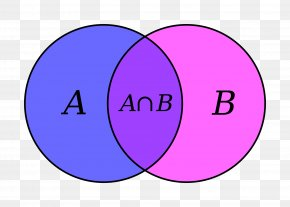
\includegraphics[width=\textwidth]{img/inclusion-exclusion.jpg}
      \caption*{Source: \href{https://bit.ly/3D8dqBo}{https://bit.ly/3D8dqBo}}
    \end{figure}
  \end{columns}
\end{frame}

\begin{frame}{Exercise: Sexagesimal numbers}
  \begin{columns}
    \column{0.5\textwidth}
    \begin{itemize}
      \item What is Sexagesimal system?
      \item Instead of having 10 symbols representing the digits (0,1,2,3,4,5,6,7,8,9), they have \textit{60} symbols representing a digits
      \item Then every 60 they carry one digit
    \end{itemize}
    \column{0.5\textwidth}
    \begin{figure}
      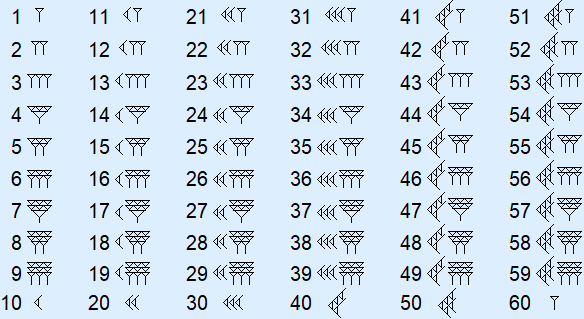
\includegraphics[width=\textwidth]{img/babylonian-numerical.png}
      \caption*{Babylonian numerals (Source: \href{https://www.dr-aart.nl/Arithmetic-roman-binary-octal-and-babylonian-numerals.html}{Dr. Aart})}
    \end{figure}
  \end{columns}
\end{frame}

\begin{frame}{Exercise: Sexagesimal numbers}
  \begin{itemize}
    \item For example, for the number represented below:
    \item The digits are 1,57,46,40
    \item So the number representing is\\ $1 \times 60^3 + 57 \times 60^2 + 46\times 60 + 40 = 424000$
  \end{itemize}
  \begin{figure}
    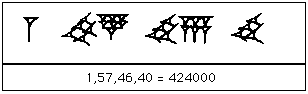
\includegraphics[width=0.6\textwidth]{img/babylonian-numer-example.png}
    \caption*{Source : \href{https://mathshistory.st-andrews.ac.uk/HistTopics/Babylonian_numerals/}{MacTour}}
  \end{figure}
\end{frame}

\begin{frame}{Exercise: Sexagesimal numbers}
  \begin{itemize}
    \item Now let's write a program that converts a decimal number into sexagesimal number
    \item Instead of those funny numerals in the previous table, we shall use the usually 0-59 separated by comma to represent the sexagesimal digit
    \item For example, 424000 in previous example will be written as {1,57,46,40}
    \item Some more examples:
  \end{itemize}
  \begin{table}[]
    \begin{tabular}{llllll}
    Base 10 & 1343    & 6948    & 67    & 382    & 23432   \\
    Base 60 & 0,22,23 & 1,55,48 & 0,1,7 & 0,6,22 & 6,30,32
    \end{tabular}
    \end{table}
\end{frame}

\begin{frame}[fragile]{Exercise: Sexagesimal number}
  \begin{exampleblock}{Problem}
    You have two task in this exercise:
      \begin{enumerate}
        \item Given a number in sexagesimal representation $\{d_1,d_2,d_3\}$, where $0\leq d_1,d_2,d_3\leq 59$, convert the number into base 10
      \end{enumerate}
  \end{exampleblock}
  \begin{exampleblock}{Example:}
    \texttt{6 30 32} in base-60 is \texttt{23432} in base-10 and \texttt{0 6 22} base-60 is \texttt{382} and so on
\begin{lstlisting}[language=bash]
    Example 1:      Example 2:      Example 3:
    ./main          ./main          ./main
    6 30 32         0 6 22          1 55 48
    23432           382             6948
\end{lstlisting} 
\end{exampleblock}
  
\end{frame}


\begin{frame}[fragile]{Exercise: Sexagesimal number}
  \begin{exampleblock}{Problem}
      \begin{enumerate}
        \setcounter{enumi}{1}
        \item Given a integer $N$ in base-10 representation, where $0 \leq N <  60^4$, return a 3 digit base-60 representation of the number
      \end{enumerate}
  \end{exampleblock}
  \begin{exampleblock}{Example:}
  \texttt{23432} in base-10 is \texttt{6 30 32}, \texttt{1343} is \texttt{0 22 23} and so on
\begin{lstlisting}[language=bash]
    Example 1:      Example 2:      Example 3:
    ./main          ./main          ./main
    23432           1343            67
    6 30 32         0 22 23         0 1 7
\end{lstlisting}
  \end{exampleblock}
\end{frame}

\begin{frame}{Number system}
  \begin{itemize}
    \item In fact, what the previous exercise illustrates is the idea of a \textbf{number system}
    \item In short, the same number can be written in vastly different ways, depending on where you choose to carry you digit
  \end{itemize}
\end{frame}

\section{Number system}
\begin{frame}{Number system}
  \begin{itemize}
    \item To illustrate this, let's consider the number 37
    \item What do we actually mean by 37?
    \item Actually we meant:
    \begin{align*}
      37 = 3 \cdot 10 + 7
    \end{align*}
    \item Similarly, when we write 139
    \begin{align*}
      139 = 1 \cdot 10^2 + 3 \cdot 10 + 9
    \end{align*}
  \end{itemize}
\end{frame}

\begin{frame}{Number system}
  \begin{itemize}
    \item In general, if we write a $m$ digit number as:
    \begin{align*}
      n = a_{m-1} a_{m-2} a_{m-3} \cdots a_{2} a_{1} a_{0}
    \end{align*}
    We mean:
    \begin{align*}
      n = a_{m-1} \cdot 10^{m-1} + a_{m-2} \cdot 10^{m-2} + \cdots + a_{2} \cdot 10^2 + a_{1} \cdot 10^{1} + a_{0}
    \end{align*}
    \textbf{This is what we meant by expressing a number in base 10}
  \end{itemize}
\end{frame}

\begin{frame}{Number system}
  \begin{itemize}
    \item To give a concrete example, consider a 3 digit number $n=293$
    \item Then $n=a_2 a_1 a_0$, with $a_2 = 2, a_1 = 9, a_0 = 3$
    \item Substituting it back to our expression:
    \begin{align*}
      n &= a_{2} \cdot 10^{2} + a_{1} \cdot 10^{1} +  a_{0}\\
      &= 2 \cdot 10^{2} + 9 \cdot 10^{1} + 3
    \end{align*}
    As expected
  \end{itemize}
\end{frame}

\begin{frame}{Number system}
  \begin{itemize}
    \item But why choose $10$? What if we choose to use another number instead of 10?
    \item Let's choose $2$ for example. Then for $n=5$:
    \begin{align*}
      5 = 1\cdot 2^2 + 0\cdot 2^1 + 1
    \end{align*}
    \item In this case, we write $5=101_2$ here the subscript $2$ means we are using 2 instead of 10
    \item In fact this is called \textbf{binary numbers}
  \end{itemize}  
\end{frame}

\begin{frame}{Number system}
  \begin{definition}[Binary numbers]
    Let $n$ be a positive integer. Then we can write $n$ in the following way:
    \begin{align*}
      n =  a_{m-1} \cdot 2^{m-1} + a_{m-2} \cdot 2^{m-2} + \cdots + a_{2} \cdot 2^2 + a_{1} \cdot 2^{1} + a_{0}
    \end{align*}
    where $a_i$ is either 0 or 1 for $0\leq i \leq m-1$. We say $n$ is a $m$ digit binary number and $a_i$ are the $i+1$th digits of $n$. Furthermore, we say $n = (a_{m-1}a_{m-2} \cdots a_{1} a_{0})_2$ is the \textbf{binary representation} of $n$ in base $2$
  \end{definition}
\end{frame}

\begin{frame}{Number system}
  \begin{itemize}
    \item For example, $n=19$:
    \begin{align*}
      19 = 1 \cdot 2^4 + 0 \cdot 2^3 + 0 \cdot 2^2 + 1 \cdot 2^1 + 1
    \end{align*}
    \item So $n=19$ is a 5 digit binary number 
    \item Also $a_0=1,a_1=1,a_2=0,a_3=0,a_4=1$ are the 1st, 2nd, 3rd, ..., 5th digits of $n$ in base 2. 
    \item Furthermore, the binary representation of $n=19$ is $10011_2$
  \end{itemize}
\end{frame}

\begin{frame}[fragile]{Number system}
  \begin{itemize}
    \item We now introduce an algorithm for finding the binary representation of $n$ in base 2
    \begin{exampleblock}{Algorithm (Binary number by short divison)}
      Let $m$ be an integer, the remainder of $m$ divided by 2 is $m \% 2$. Then the following algorithm gives the binary representation for an integer $n$:
      \begin{enumerate}
        \item $n_0 = n$
        \item $a_i = n_i \% 2$
        \item $n_{i+1} = (n_i - a_i) / 2$
        \item repeat 2,3 until $n_i = 0$ 
      \end{enumerate}
    \end{exampleblock}
  \end{itemize}
\end{frame}

\begin{frame}{Number system}
  \begin{itemize}
    \item Example of executing the algorithm by hand:
    \begin{figure}
      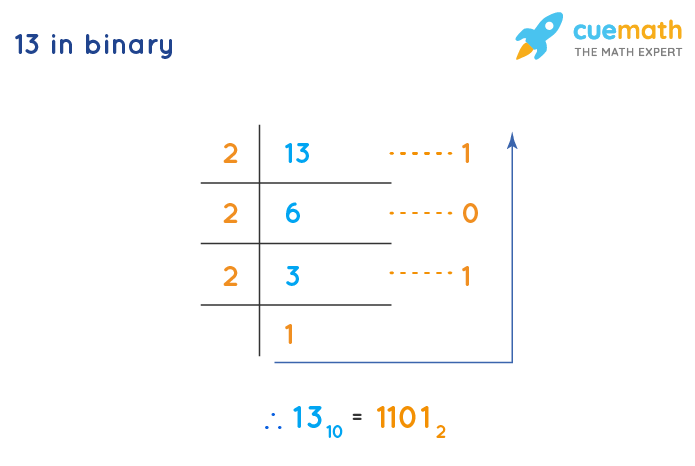
\includegraphics[width=0.5\textwidth]{img/binary-decimal-short-div.png}
      \caption*{Source: \href{https://www.cuemath.com/numbers/13-in-binary/}{Cuemath}}
    \end{figure}
  \end{itemize}
\end{frame}

\begin{frame}{Number system}
  \textbf{Exercise:}
  \begin{enumerate}
    \item Convert the following numbers into binary: 16,93,34,11
    \item What is the last digit in the binary representation of the following numbers (Hint: You can read out the ans directly): 19,30,44,21
    \item Convert the following binary numbers back to deciaml: $101_2, 1011_2,111_2,1111_2$
  \end{enumerate}
\end{frame}

\begin{frame}[fragile]{Number system}
  \begin{itemize}
    \item Here is a code that does decimal to binary conversion
  \end{itemize}
\begin{lstlisting}[language=python]
n = int(input('Enter an integer: '))
a = [] # List storing the digits

while n != 0:
  ai = n%2      # Step 2
  a.append(ai)  # Add i th digit on list
  n = (n-ai)//2 # Step 3

a = a[::-1] # Reverse the list (e.g. [1,0,1,1] -> [1,1,0,1])
print(a) # Print the digits
\end{lstlisting}
\end{frame}

\begin{frame}{Number system}
  \begin{itemize}
    \item We can extend the definition to include arbitary bases:
  \end{itemize}
  \begin{definition}[Base $b$ numbers]
    Let $n$ be a positive integer. Then we can write $n$ in the following way:
    \begin{align*}
      n =  a_{m-1} \cdot b^{m-1} + a_{m-2} \cdot b^{m-2} + \cdots + a_{2} \cdot b^2 + a_{1} \cdot b^{1} + a_{0}
    \end{align*}
    where $a_i$ is from $0$ to $b-1$ for $0\leq i \leq m-1$. We say $n$ is a $m$ digit number in base $b$ and $a_i$ are the $i+1$th digits of $n$. Furthermore, we say $n = (a_{m-1}a_{m-2} \cdots a_{1} a_{0})_b$ is the representation of $n$ in base $b$
  \end{definition}
\end{frame}

\begin{frame}{Number system}
  \begin{exampleblock}{Example (Base 16)}
    Another often used base in computer science is base 16. By our previous definition, the digits of base 16 numbers ranges from $0-15$ and $b=16$. For example, the number 57 is represented in base 16 as:
    \begin{align*}
      57 = 3\cdot 16^1 + 9 
    \end{align*}
    Hence, $57=(39)_{16}$
  \end{exampleblock}
\end{frame}

\begin{frame}{Number system}
  \begin{exampleblock}{Example (Base 16) Cont.}
    What about 31? Note that:
    \begin{align*}
      31 = 1\cdot 16^1 + 15
    \end{align*}
    Hence $31 = ([1][15])_{16}$. Here I use $[\cdots]$ to represent a digit in base 16. Note that $15$ here is treated as a digit in base $16$
  \end{exampleblock}
\end{frame}

\begin{frame}{Number system}
  \begin{exampleblock}{Example (Base 16) Cont.}
    This notation is clumsy, so in practice people use another set of conventions to denote digits from 10 to 15:
    
    \begin{table}
    \begin{tabular}{ccccccc}
      
      Digit & 10 & 11 & 12 & 13 & 14 & 15\\
      Symbol& A & B & C & D & E & F \\  
    \end{tabular}
  \end{table}

    Hence, the number $31 = (1F)_{16}$ in this new notation 
  \end{exampleblock}
\end{frame}

\begin{frame}{Number system}
  \begin{exampleblock}{Exercise}
    \begin{enumerate}
      \item Convert the following numbers from decimal to base 16: 372, 271,31,39,86
      \item Convert the following binary numbers to base 16: $(10110101)_{2}, (111001010110)_{2},(0100110010)_2$
      \item Convert the following base 16 numbers to binary and decimal: $(1A)_{16},(43)_{16},(9E)_{16},(2D)_{16},(7B)_{16}$
    \end{enumerate}
  \end{exampleblock}
\end{frame}

\section{More on binary numbers}
\begin{frame}{More on binary numbers}
  \begin{itemize}
    \item Since binary numbers are of great importance in computer science, let's discuss more about it
    \item First, let's introduce some notations
  \end{itemize}
\end{frame}

\begin{frame}[fragile]{Denoting binary in Python}
  \begin{itemize}
    \item In python, we denote a binary number like this : \texttt{0b<binary digits>}
    \item For example, \texttt{17 = 0b10001} because $17 = 1\times 2^4 + 0 \times 2^3 + 0 \times 2^2 + 0 \times 2^1 + 1 \times 1$
    
    \item So in python we writes:
\begin{lstlisting}[language=python]
x = 0b10001 # same as x = 17
\end{lstlisting}
  \end{itemize}
  \begin{exampleblock}{Exercise}
    Convert the following numbers from binary to decimal and check your answer against that by python:\\
    \texttt{0b01010, 0b11011, 0b01010, 0b10011}
  \end{exampleblock}
\end{frame}

\begin{frame}[fragile]{Denoting hexadecimal in Python}
  \begin{itemize}
    \item Similarly we can denote hexadecimal numbers like this: \texttt{0x<hex digits>}
    \item For example, \texttt{17=0x11} because $17 = 1 \times 16^1 + 1$
    \item So in python we write
\begin{lstlisting}[language=python]
x = 0x11 # same as x = 17
\end{lstlisting}
  \end{itemize}
  \begin{exampleblock}{Exercise}
    Convert the following numbers from hexadecimal to decimal and check your answer against that by python:\\
    \texttt{0xA31, 0xD13, 0x12C, 0x14}
  \end{exampleblock}
\end{frame}

\section{Bit and byte}
\begin{frame}{Bits and Bytes}
  \begin{itemize}
    \item Using the ideas of binary numbers, we can talk about bit and bytes
    \item You may think every bits as a 0 or 1 in a binary number 
    \item More generally, we can also use bits to represent binary states 
    \item For example, we can say a game character is dead if the \texttt{isAlive} status is \texttt{0} and alive if it is \texttt{1}
    \item In the following slides, we will talk about how bits and byte relates to storage capacities
  \end{itemize}
\end{frame}


\begin{frame}{Bit}
  \begin{itemize}
    \item \textbf{Bit} is the most basic unit of information in computing and digital communications.
    \item The short hand is \textbf{b}
    \item It represent a \textbf{logical state} of \textit{either true or false (0 or 1)} 
    \item Information are stored in computer as an array of bits
  \end{itemize}
\end{frame}

\begin{frame}{Bit}
  \begin{columns}
    \column{0.6\textwidth}
    \begin{itemize}
      \item Obviously, for a \textit{fixed length} of bits, there is a \textit{limited number of states} storable. That define the "maximum storage capacity" of that array 
      \item For example, consider a storage area of 2 bits (represented by the two light bulbs) on the right
      \item Since there are only two light bulbs, it follows there can only be 4 states: ${(0,0),(0,1),(1,0),(1,1)}$
    \end{itemize}
    \column{0.4\textwidth}
    \begin{figure}
      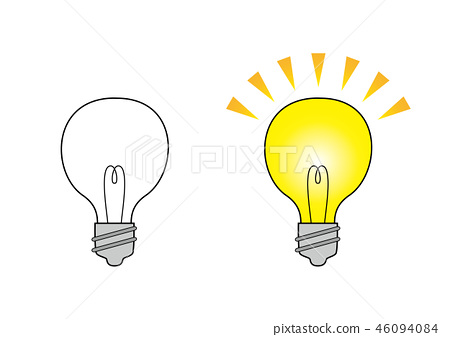
\includegraphics[width=\textwidth]{img/two-light-bulb.jpg}
      \caption*{Source: \href{https://www.pixtastock.com/illustration/46094084}{PIXTA}}
    \end{figure}
  \end{columns}
  
\end{frame}

\begin{frame}{Bit}
  \begin{itemize}
    \item In general, suppose we have $N$ bits. Then each of the bits can either be on or off (1 or 0), so there are:
    \begin{align*}
      \overbrace{2\times 2 \times \cdots 2 \times 2}^{\text{N times}} = 2^N
    \end{align*}
    states storable in an array of $N$ bits
    \item This result will be useful when we discuss about overflow and size limits in later chapters
    \item Just remember for now variables like \texttt{int}, \texttt{float} cannot store every value in the world, they are limited by the number of states available for a $N$ bit number
  \end{itemize}
\end{frame}

\begin{frame}{Byte}
  \begin{itemize}
    \item A \textbf{byte} is defined to be 8 bit 
    \item E.g. 4 byte storage is 8x4=32 bit large
    \item Short form: \textbf{B}
    \item E.g. 16B = 16 byte = 128 bit
  \end{itemize}
\end{frame}

\begin{frame}{Kilo, Mega, Giga and Tera}

  \begin{itemize}
    \item In SI units, 1 kilo is 1000
    \item But in computer science 1 kilo is actually $2^{10} = 1024$
    \item For example:
    \item 1 kilobyte (KB) = 1024 B
    \item 1 megabyte (MB) = 1024 KB
    \item 1 gigabyte (GB) = 1024 MB
    \item 1 terabyte (TB) = 1024 GB
  \end{itemize}
\end{frame}

\begin{frame}{Kilo, Mega, Giga and Tera}
  \begin{exampleblock}{Exercise}
    \begin{enumerate}
      \item A USB drive has a size of 4GB. A typical image has size of 6MB. Roughly how many images can a USB store?
      \item James was trying to download a file of 132KB from the internet. He did a speed test on his network and found that is download speed is 57.78Mbps (Mega\textit{bit} per second). Estimate how long is needed for him to download the file.
      \item Now he has to upload a file of 0.0001TB through the internet. If his upload speed is 23.69Mbps, how long would it takes to upload the file?
    \end{enumerate}
  \end{exampleblock}
\end{frame}

\end{document}
